\newpage
\section{Aufbau}
\label{sec:Aufbau}
Der hier untersuchte Si-Streifendetektor (EASy) der Firma Alibava besteht aus drei Komponenten, Kontrall-, Detektoreinheit und Computer mit Steuer-Software.

\subsection{Detektoreinheit}
\label{sec:Detektoreinheit}
 Als Detektoreinheit wierd der Si-Streifenhalbleiter und die Ausleseelektronik
 zusammengefasst. Dabei besteht der \SI{300}{\micro\meter} dicke Si-Detektor
 aus 128 einzelnen p-dotierten Streifen in dem n-dotierten Silizium.  Dieser
 Aufbau ist in Abbildung \ref{fig:schema} zu erkennen.
 \begin{figure}[htb]
   \centering
   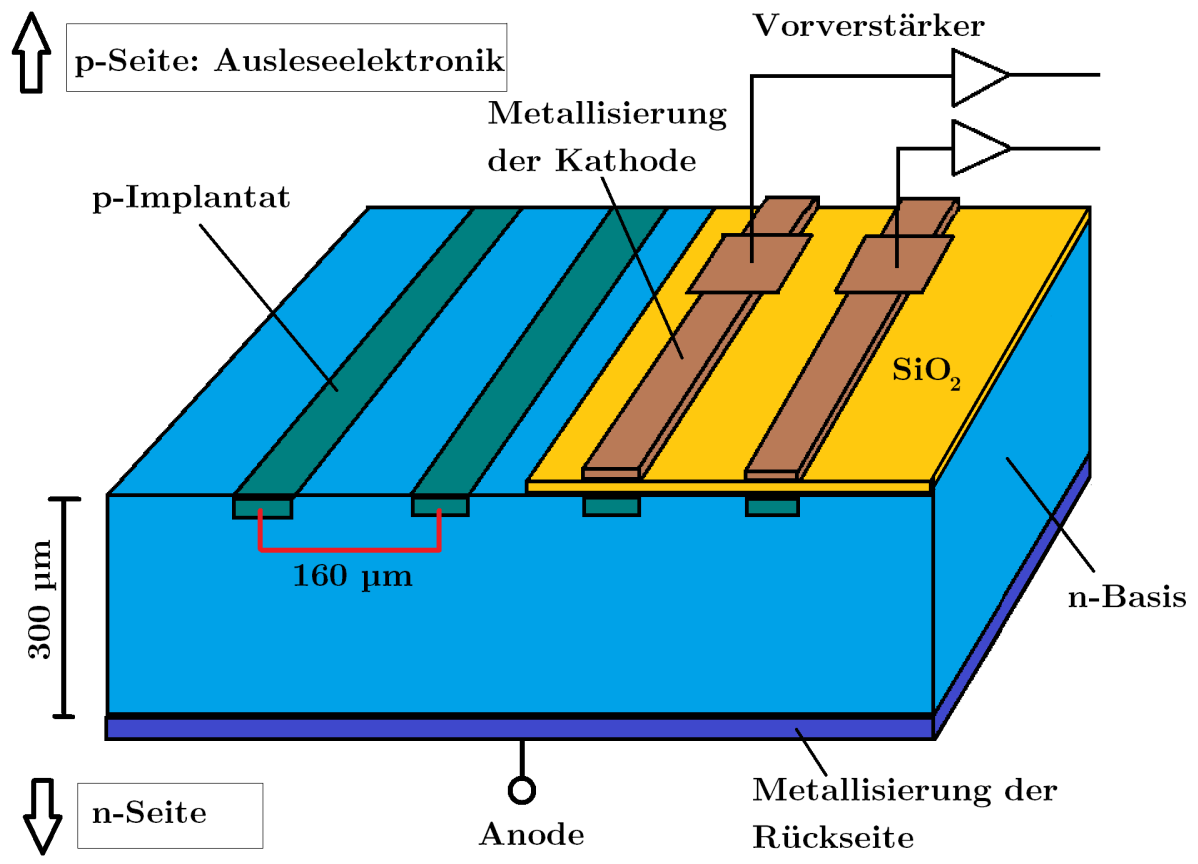
\includegraphics[width=0.7\textwidth]{images/Schema.png}
   \caption{Schematische Darstellung eines Si-Streifensensors mit Spannungsanschluss \cite{anleitung}.}
   \label{fig:schema}
 \end{figure}
Eine Schicht aus Siliziumoxid sorgt dafür, dass kein Signal aus den p-Implantaten
auf überschlägt. Jeder Streifen ist durch das Wirebonding mit ein Pad und weiter
einem ohmschen Widerstand
verbunden. Dieser wiederum ist an einen Bias Ring zur Spannungsversorgung gekoppelt.
Um den Bias Ring ist ein Guard Ring zur Vermeidung von Spannungsüberschlägen vom Bias
Ring zur Ausleseelektronik angebracht. In Abbildung \ref{fig:streifen} ist dies an
einer makroskopischen Aufnahme deutlich gemacht.
\begin{figure}[htb]
  \centering
  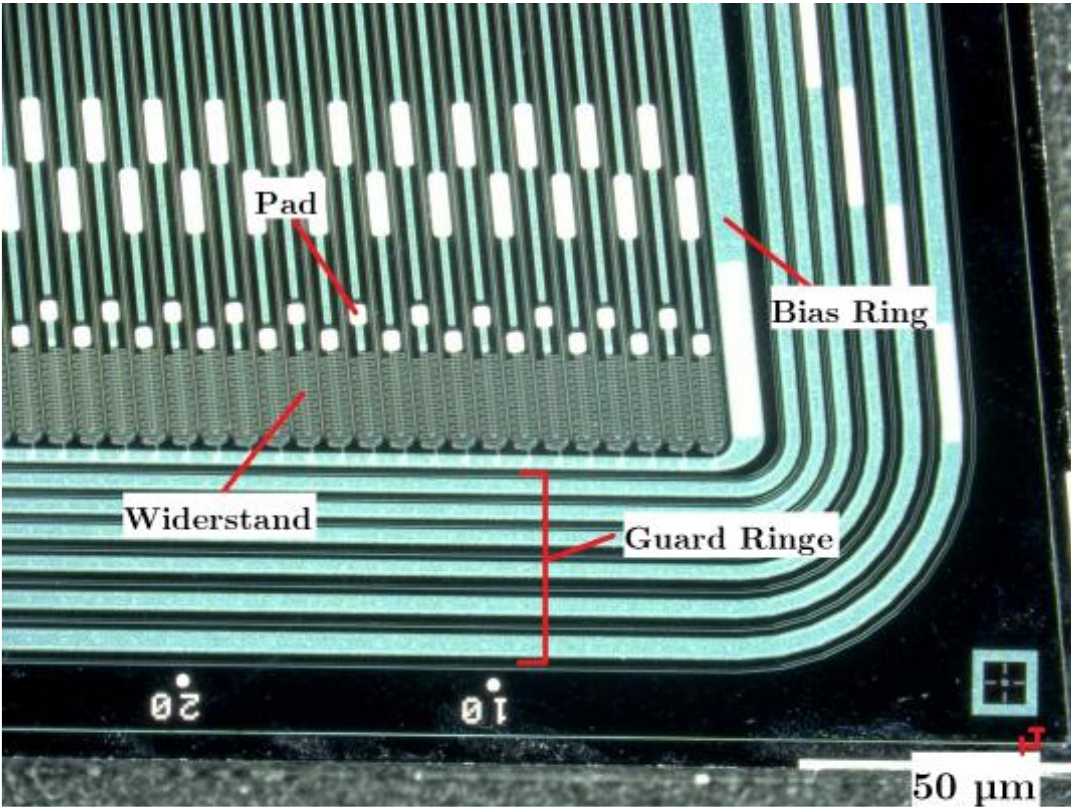
\includegraphics[width=0.7\textwidth]{images/Sensor.png}
  \caption{Makroskopische Aufnahmne eines Streifen-Detektors mit entsprechender kennzeichnung der einzelnen Komponenten \cite{anleitung}.}
  \label{fig:streifen}
\end{figure}
Die Informationen aus den einzelnen Streifen nach Durchgang eines geladenen
Teilchens wird durch einen Auslesechip zuerst verstärkt und danach in
Spannungssignale umgewandelt. Dann werden die Signale in eine Pipeline geschickt.

Diese Funktionsweise funktioniert, wie in \ref{sec:Theorie} erst richtig, wenn der
Halbleiterdetektor follständig depletiert ist. Bei dem EASy liegt dazu
$U_\text{Dep}$ bei ungefähr \SIrange{60}{80}{\volt}.

Aus Abbildung \ref{fig:Gehäuse}ist das äußere Gehäuse des Detektors zu entnehmen.
\begin{figure}[htb]
  \centering
  \includegraphics[width=0.7\textwidth]{images/Gehäuse.png}
  \caption{Fotographie des EASy Gehäuses mit integriertem Laser und Carbon-Plätchen, sowie den einzelnen Anschlüssen \cite{anleitung}.}
  \label{fig:Gehäuse}
\end{figure}


\section{Durchführung}
\label{sec:Durchführung}
